\chapter{Versuchsaufbau und -ablauf}\label{Kapitel 3}
\interfootnotelinepenalty 10000
Das folgende Kapitel beschreibt die Ziele der Messung, Versuchsaufbau und -durchf"uhrung. Ziel der Messung ist die Untersuchung des Skalierungsverhaltens der ausgew"ahlten HPC-Benchmarks auf dem Bramble. Die Ergebnisse sollen unter Vergleichswerte des Bramble gegen"uber einem Supercomputer liefern. Dazu wird der Bramble an Hand der Messwerte in die TOP500- und Green 500-Listen eingeordnet (vgl. Kap. \ref{Rankings}). 

\section{Zielsetzung}

Von der Messung werden detaillierte Erkenntnisse "uber das Skalierungsverhalten von HPLinpack und Whetstone auf dem Bramble mit 20 RPi-Nodes erwartet. Alle Messungen werden auf 1 -- n RPi-Nodes des Bramble durchgef"uhrt mit n = 20. Die Messungen werden zwei Mal durchgef"uhrt: Zuerst mit Netzwerkanschluss der gerade nicht beteiligten RPi-Nodes an den Bramble-Server, danach ohne. 

Als Output-Parameter werden der Energieverbrauch des Bramble und die jeweils Benchmark-spezifischen Load-Generatoren betrachtet. Der Stromverbrauch wird durch ein Strommessger"at ermittelt, das an den Bramble-Server angeschlossen wird. Die Benchmark-spezifischen Load-Generatoren sich nat"urlich an den vom jeweiligen Programm vorgegebenen Parametern: HPLinpack liefert 4 Ma\ss zahlen f"ur die CPU-Performance eines Rechners/Rechnersystems. $R_{max}$ entspricht der Performance in GFLOPS bei Ausf"uhrung des gr"o\ss ten Problems, $N_{max}$ bezeichnet das gr"osste ausgef"uhrte Problem, $N_{1/2}$ die Problemgr"o\ss e bei halber $R_{max}$-Rate und $R_{peak}$ die theoretische Peak-Performance in GFLOPS. Whetstone liefert drei Kennzahlen f"ur die CPU-Performance: MWIPS (Millions of Whetstone Instructions per Second), davon abgeleitet MFLOPS f"ur die Ausf"uhrung der Flie\ss punkt-Operationen und MIPS (Millions of Instructions per Second) f"ur die Integer-Tests. 

\section{Aufbau und Art der Messung}\label{Aufbau}

F"ur den Versuchsaufbau stellen sich zwei grundlegende Fragen: Welcher Art ist die Messung und welche Voraussetzungen m"ussen hierf"ur gelten? 

Die durchzuf"uhrende Messung hat zwei Ausgabeparameter: Energieverbrauch und die jeweils Benchmark-spezifischen Ausgabewerte. F"ur den Versuchsaufbau sind daher folgende Aspekte von Bedeutung: Zeitsynchronisation der RPi-Nodes, Skalierung der Messung auf 1 -- n RPi-Nodes, automatisierte Durchf"uhrung der Messung f"ur 1 -- n RPi-Nodes, Einlesen der Messwerte in eine geeignete Datenstruktur, Ausgabe und Aufbereitung der Messwerte. 

Um sich mit den grundlegenden Funktionalit"aten vertraut zu machen, wurden die ausgew"ahlten Benchmarks zun"achst auf einem RPi-Einzelrechner ausgef"uhrt. Dabei wurden schnell die grundlegenden Unterschiede zum Bramble deutlich, vor allem hinsichtlich des Filesystems. Dies wirkt sich auf die Auswahl der Benchmark-Implementierungen aus: Z.B. ist die Ausf"uhrung von HPLinpack auf einem Einzelrechner nicht m"oglich. Auch der Versuchsaufbau und die Ausf"uhrung der Benchmarks sind hiervon betroffen: Zeitsynchronisation und Skalierung der Messung auf 1 -- n Nodes sind bei einem RPi-Einzelrechner nicht notwendig, wohl aber bei einem Cluster. 

Da der Schwerpunkt auf dem Skalierungsverhalten der Benchmarks auf dem Bramble liegt, wird der Versuchsaufbau f"ur den RPi-Einzelrechner im Folgenden nur kurz skizziert. Die Ergebnisse von Linpack 100 und Whetstone auf dem RPi-Einzelrechner sind im Anhang dokumentiert (vgl. Kap. \ref{Ergebnisse_RPi}).  

\subsection{Versuchsaufbau Ri-Einzelrechner}\label{RPi-Versuchsaufbau}

F"ur die meisten RPi-User stellen sich nach Auswahl, Installation und Konfiguration des Betriebssystems zwei Fragen nach Swap Space und "Ubertakten. Beides liegt auf der Hand, da der RPi Modell B nur "uber einen Arbeitsspeicher von 512 MB verf"ugt. Die CPU-Leistung ist mit 700 MHz ebenfalls nicht eher niedrig. 

Im Praxisbetrieb zahlreicher User zeigte sich, dass ein "Ubertakten der CPU auf bis auf 1 GHz anscheinend gefahrlos m"oglich ist. In der Konsequenz entschloss sich die Raspberry Pi Foundation, den Verlust der Garantieleistung bei "Ubertaktung aufzuheben. Beim hier verwendeten Testger"at wurde dennoch auf das "Ubertakten verzichtet, um die Vergleichbarkeit mit anderen RPi-Einzelrechnern und dem Bramble sicherzustellen\footnote{Es erscheint wenig zielf"uhrend, die Komponente zu tunen, deren Performance man mittels Benchmarking evaluieren m"ochte. F"ur eine sp"atere Untersuchung ist dies jedoch nicht ausgeschlossen. Z.B. w"are es interessant zu ermitteln, ob man den relativ hohen Stromverbrauch des Bramble bei Niedriglast (vgl. \cite{kli13}) durch Untertakten der einzelnen CPUs senken kann.}.

Das gew"ahlte Betriebssystem Raspbian verwendet standardm"a\ss ig eine Swap-Datei (\verb+/var/swap+), die den Adressraum des Arbeitsspeichers bei "Uberlast erweitert. Hierbei gibt es zwei Probleme: Erstens k"onnten st"andige Schreibzugriffe auf Dauer die SD-Karte besch"adigen\footnote{Vgl. \cite{pow12}.}. Au\ss erdem sind Schreibzugriffe auf die SD-Karte sehr langsam, was die Performanz des Systems bei hoher Arbeitsspeicherlast beeintr"achtigen kann. Aus diesem Grund wurde entschieden, zun"achst auf die Nutzung der Swap-Datei zu verzichten\footnote{Die Swap-Datei kann mit dem Befehl \texttt{sudo update-rc.d dphys-swapfile remove} deaktiviert werden. Eine weitere M"oglichkeit des Swapping ist die Verwendung von zRAM, sodass ein Teil des Arbeitsspeichers komprimiert und als Swap Space genutzt wird (vgl. \cite{pow12}). Die Allokierung einer auf Unix-Systemen "ublicherweise genutzten Swap-Partition ist nicht sinnvoll, da auch hierdurch die Lebensdauer der SD-Karte durch h"aufige Schreibzugriffe verk"urzt wird.}.

\subsection{Versuchsaufbau Bramble}\label{Bramble-Versuchsaufbau}

Das folgende Komponentendiagramm (\ref{fig:Komponentendiagramm}) zeigt den Versuchsaufbau pro Messreihe, der als \textit{ExperimentSuite} bezeichnet wird Das Diagramm orientiert sich an den Aspekten, an die systemkritisch f"ur die Versuchsdurchf"uhrung sind: \textit{Stromversorgung} und \textit{Netzwerkanschluss} des Bramble, \textit{Messung des Stromverbrauchs} mit dem Strommessger"at, \textit{Loggen des gemessenen Stromverbrauchs} und \textit{Upload der Messergebnisse} in eine MySQL-Datenbank auf dem Bramble-Server. 
\begin{figure}[htb]
  \centering
  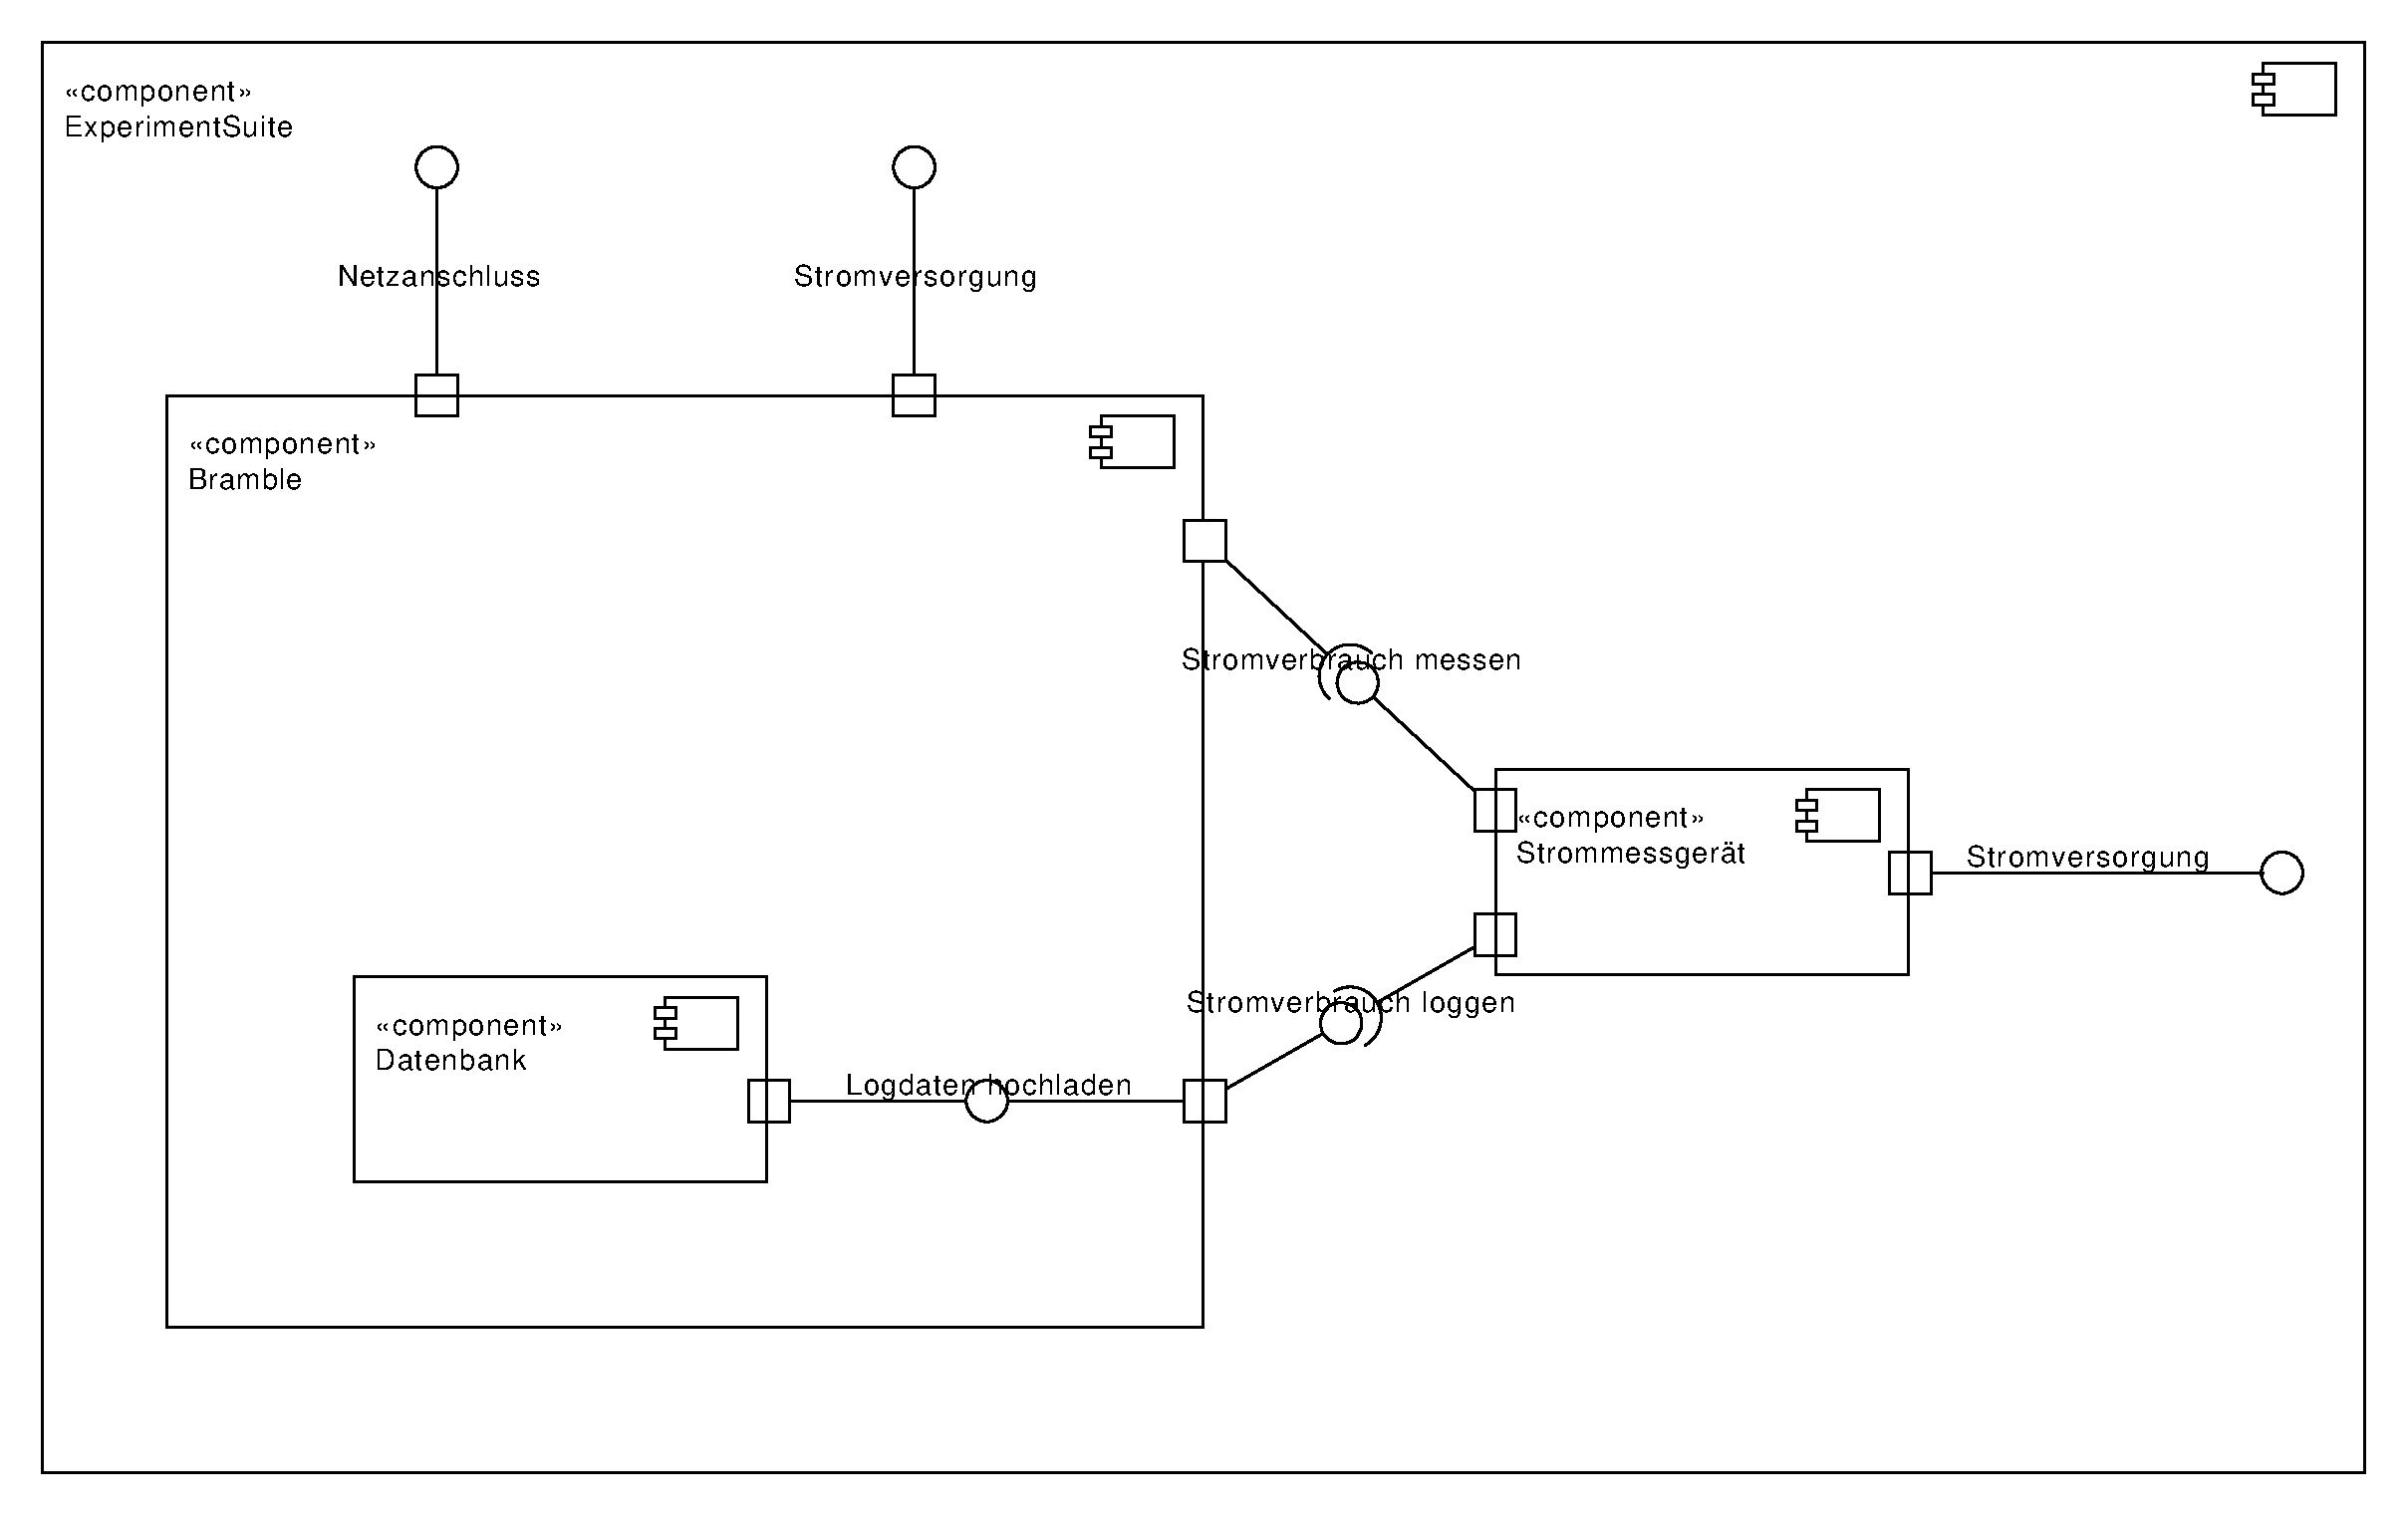
\includegraphics[width=\textwidth]{komponentendiagramm2.pdf}\\ 
  \caption{Komponentendiagramm des Versuchsaufbaus.}
  \label{fig:Komponentendiagramm}		
\end{figure}

\subsection{Skalierung der Messung auf 1 -- n RPi-Nodes}

Die Benchmark-generierte Workload und die Messung dieser Ergebnisse findet im Inneren der Komponente \textit{Bramble} statt. Auf dem Bramble-Server wird ein Prozess angesto\ss en, der den jeweiligen Benchmark auf 1 -- 20 RPi-Nodes ausf"uhrt, zun"achst ohne und dann mit Stromanschluss der gerade nicht beteiligten RPi-Nodes. Das folgende Aktivit"atsdiagramm zeigt, welche Schritte aus Benutzersicht f"ur die Durchf"uhrung einer ExperimentSuite erforderlich sind. Dabei wird mir n = 20 RPi-Nodes begonnen und einmal "uber alle Nodes von 20 -- 1 iteriert. Danach wird die zweite Messung ebenfalls als Iteration "uber die RPi-Nodes 20 -- 1 durchgef"uhrt, wobei nach jedem Iterationsschritt der RPi-Node abgeschaltet wird. Dieser Aufbau ist in einem Aktivit"atsdiagramm dargestellt (vgl. \ref{fig:Aktivitaetsdiagramm}).  
\begin{figure}[htb]
  \centering
  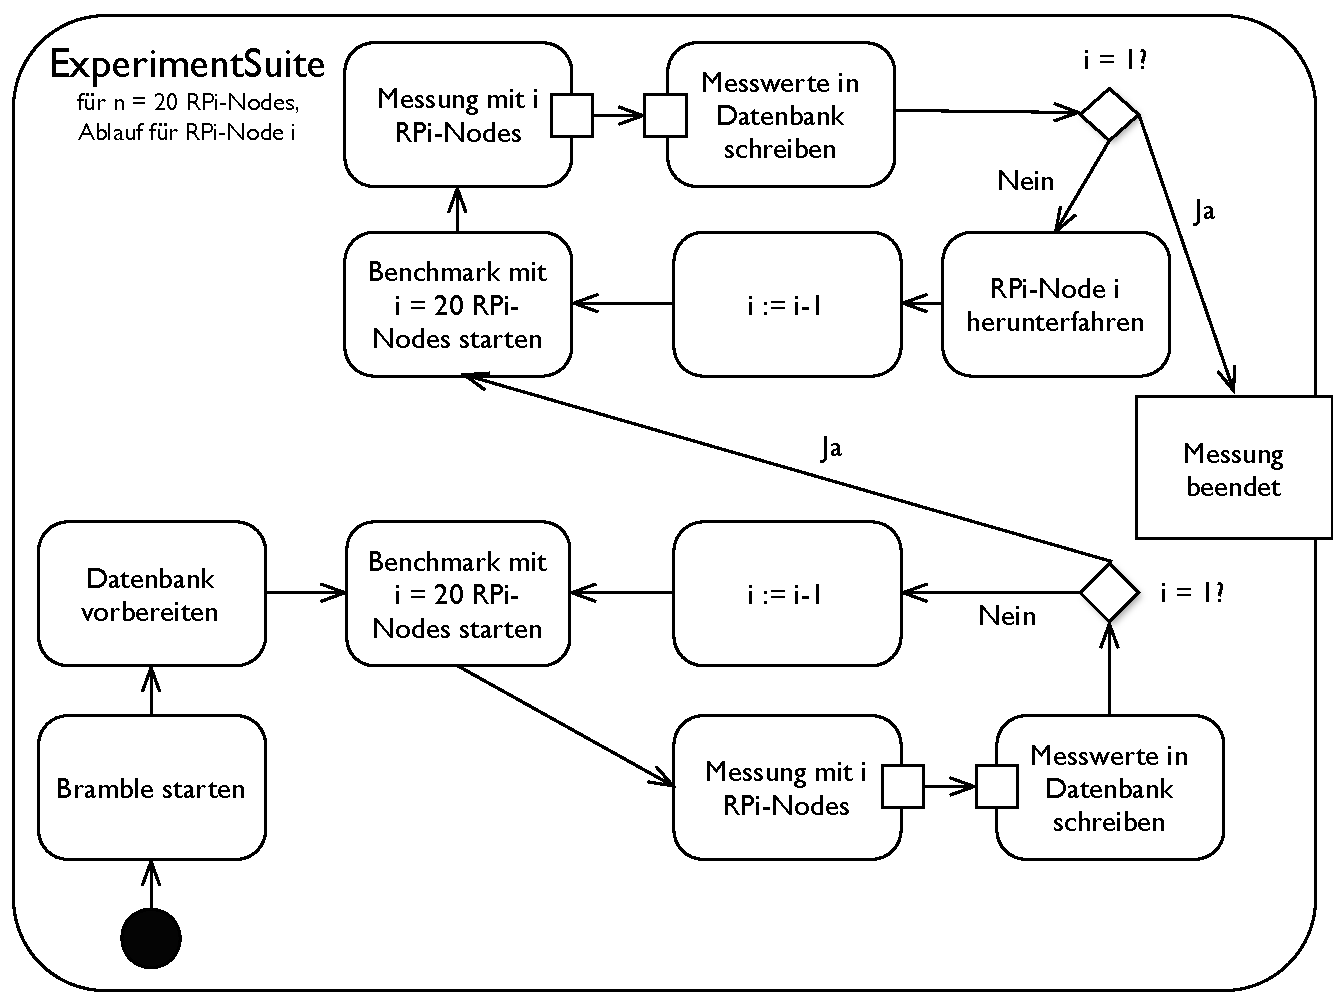
\includegraphics[width=0.7\textwidth]{aktivitaetsdiagramm2.pdf}\\ 
  \caption{Aktivit"atsdiagramm der ExperimentSuite.}
  \label{fig:Aktivitaetsdiagramm}
\end{figure}

\subsection{Automatisierte Durchf"uhrung der Messung f"ur 1 -- n RPi-Nodes}

Die automatisierte Ausf"uhrung der Benchmarks erfolgt mit einem Shellskript auf dem Ausf"uhrungs-Node \texttt{pi03} (vgl. \ref{executeBenchmarksOnAllRPis.sh}). Es ist im gesharten Verzeichnis der RPi-Nodes \texttt{/srv} abgelegt und enth"alt unter anderem folgende Schritte: 
\begin{enumerate}
	\item L"osche altes Machinefile.
	\item Erstelle ein neues Machinefile mit allen RPi-Nodes von 1 -- 20 in\newline\texttt{/srv/libraries/etc/mpich-3.0.4-shared/}.
	\item Mounte das gesharte Verzeichnis \texttt{/srv} auf allen RPi-Nodes.
	\item Benutzereingabe f"ur den auszuf"uhrenden Benchmark, das Arbeitsverzeichnis und ein optionales Parameterfile. 
	\item Erstelle zwei Ausgabedateien. 
	\item F"ur alle RPi-Nodes von 20 -- 1: F"uhre den Benchmark auf n Nodes aus und logge die Ausgabe in die Ausgabedatei.
	\item Wiederhole Schritt 6 und schalte RPi-Node n nach dem Loggen der Ausgabe aus.  
\end{enumerate}

\subsection{Zeitsynchronisierung der RPi-Nodes}

Ein wichtiger Aspekt bei der parallelen Ausf"uhrung eines Programms ist die Zeitsynchronisation. Alle angesto\ss enen Berechnungen m"ussen auf allen beteiligten Knoten zum exakt selben Zeitpunkt starten, um verl"assliche Messergebnisse zu liefern. Auf einem RPi ist das kritisch, da er keine Systemuhr hat. Auf dem Bramble wird die Zeitsynchronisation der einzelnen RPi-Nodes durch einen OpenNTP-Server realisiert, der auf dem Bramble-Server installiert wurde. Die einzelnen RPi-Nodes synchronisieren sich gegen diesen Server\footnote{Vgl. \cite{kli13}.}. Die Zeitsynchronisation der RPi-Nodes ist somit auch f"ur die verteilte Ausf"uhrung der Benchmarks gew"ahrleistet. 

% TODO: 
\subsection{Einlesen der Messwerte in die Datenbank}

% TODO: 
\subsection{Ausgabe und Aufbereitung der Messwerte}

\section{Ergebnisse}\label{Ergebnisse}

Auch hier liegt der Schwerpunkt auf den Ergebnissen der Messungen von HPLinpack und Whetstone auf dem Bramble. Der RPi-Einzelrechner erreichte f"ur Linpack 100 41.31 MFLOPS. F"ur Whetstone wurden 255.154 MWIPS erreicht\footnote{Die Ergebnisdateien f"ur beide Benchmarks finden sich im Anhang unter \ref{Ergebnisse_RPi}. Die vom Autor der verwendeten Implementierung erzielten Ergebnisse auf einem RPi-Einzelrechner sind unter \url{http://www.roylongbottom.org.uk/Raspberry\%20Pi\%20Benchmarks.htm\# anchor4} zu finden.}.

\subsection{Linpack}\label{Ergebnisse Linpack}

% TODO 

\subsection{Whetstone}\label{Ergebnisse Whetstone}

% TODO 

\endinput 


